
	\section*{Harmonischer Oszillator, analytisch, Aufgabe 2.1}\label{sec:ag2.1}
	\begin{figure}[h]
		\centering
		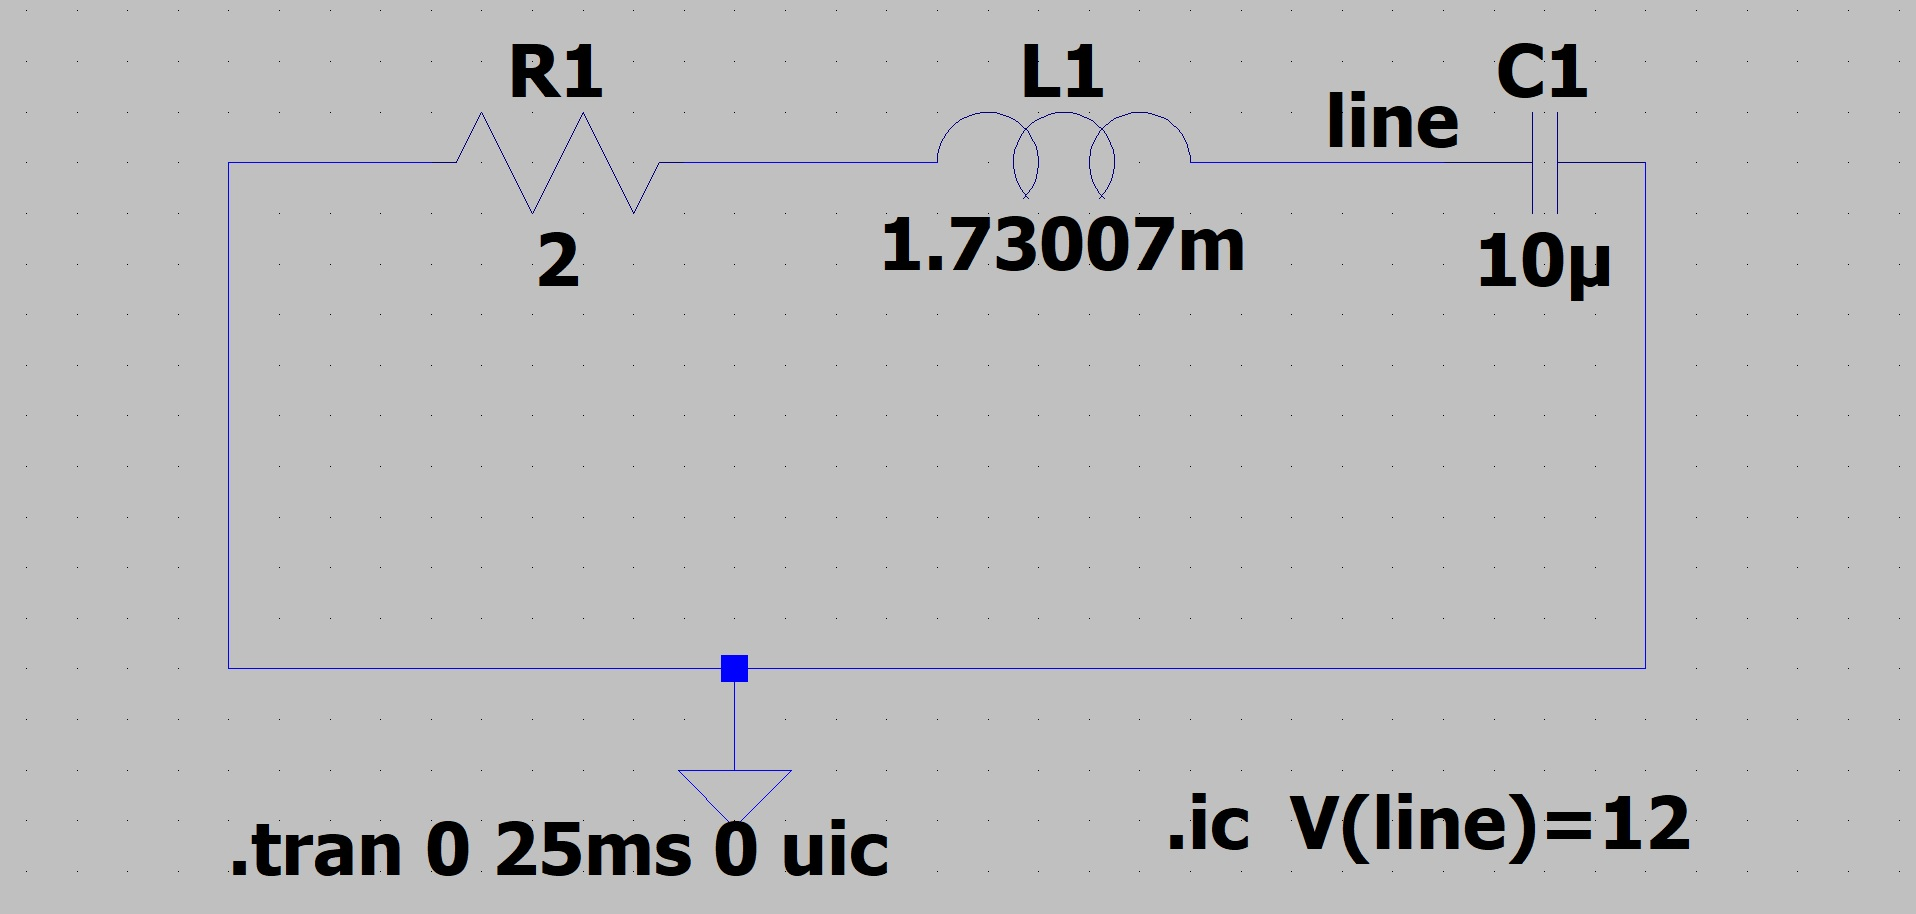
\includegraphics[width=\textwidth]{data/harmOsz}
		\caption{Gegebener harmonischer Oszillator in LT-Spice implementiert}
		\label{oszillator}
	\end{figure}
	Für die vorliegende Schaltung wird angenommen, dass am Kondensator zum Zeitpunkt $t = 0$ eine Spannung $u_\mathrm{C}(0) = 12\,$V anliegt und der Strom durch den Reihenschwingkreis $i(0) = 0\,$A beträgt. Nach dem \textsc{Kirchhoff}'schen Gesetz ergibt sich die Maschengleichung für den Schwingkreis zu $u_\mathrm{C}(t) + u_\mathrm{R}(t) + u_\mathrm{L}(t) = 0$. Aus den Spannungen für den Widerstand $u_\mathrm{R}(t) = R \: i_\mathrm{R}(t)$, die Spule $u_\mathrm{L}(t) = L\: \frac{\mathrm{d}i_\mathrm{L}}{\mathrm{d}t}(t)$ und den Kondensator $u_\mathrm{C}(t) = \frac{1}{C} \int i_\mathrm{C}(t)dt $ ergibt sich daraus die Maschengleichung in Abhängigkeit des Stromes zu 
	
	\begin{equation*}
		R\:i(t) + L\: \frac{\mathrm{d}i}{\mathrm{d}t}(t) + \frac{1}{C} \int i_\mathrm{C}(t)dt = 0.
	\end{equation*}
	
	Nach einmaligem Differenzieren nach der Zeit $t$ folgt daraus die Differentialgleichung 2. Ordnung 
	
	\begin{equation}
		R  \frac{\mathrm{d}i}{\mathrm{d}t}(t) + \frac{1}{\mathrm{C}} i(t) +  L\: \frac{\mathrm{d^2}i}{\mathrm{d}t^2}(t) = 0.
		\label{eq:it1}
	\end{equation}
	
	
	
	Die Lösung der Differentialgleichung im Falle einer gedämpften Schwingung lässt sich aus dem allgemeinen Ansatz 
	
	\begin{equation}
			i(t) = a\mathrm{e}^{(-\delta +j\omega_e)t} + b\mathrm{e}^{(-\delta - j\omega_e)t}
			\label{eq:it2}
	\end{equation}
	
	ermitteln. Hierbei bezeichnet $\delta = \frac{R}{2L}$ die Dämpfung, $\omega_0 = \sqrt{\frac{1}{LC}}$ die Resonanzkreisfrequenz und $\omega_e = \sqrt{\omega_0^2 - \delta^2}$ die gedämpfte Resonanzkreisfrequenz. Die Konstanten $a$ und $b$ werden bestimmt durch einsetzen des Anfangswertes  $i(0) = 0\,$A folgt $a + b = 0$ und somit $a = -b$.\newline
	Da zum Zeitpunkt $t = 0$ noch kein Strom fließt liegt noch keine Spannung $u_\mathrm{R}$ an dem Ohmschen Widerstand $R$ an und somit vereinfacht sich \ref{eq:it1} zu $u_\mathrm{C}(0) +  L\: \frac{\mathrm{d}i}{\mathrm{d}t}(0) = 0$ und durch einsetzen von $u_\mathrm{C}(0) = 12\,$V folgt daraus $L\frac{\mathrm{d}i}{\mathrm{d}t}(0) = -12\:$V. Einmaliges differenzieren von \ref{eq:it2} sowie einsetzen von $ i(0) = 0$ und $a = -b$ ergibt $\frac{\mathrm{d}i}{\mathrm{d}t}(0) = -j2\omega_e b$. Gleichsetzen und nach $b$ auflösen und man erhält $b = -j \frac{u_\mathrm{C}(0)}{2L\omega_e}$ und somit $a = j\frac{u_\mathrm{C}(0)}{2L\omega_e}$. Der Strom ergibt sich damit nun zu 
	
	\begin{equation}
		i(t) = j\frac{u_\mathrm{C}(0)}{2L\omega_e}\mathrm{e}^{(-\delta +j\omega_e)t} - j \frac{u_\mathrm{C}(0)}{2L\omega_e}\mathrm{e}^{(-\delta - j\omega_e)t}.
		\label{eq:it3}
	\end{equation}
	
	Durch einfaches ausmultiplizieren und nutzen der \textsc{Euler}'schen Formel 
	
	\begin{equation*}
		\mathrm{sin}(x) = \frac{\mathrm{e}^{ix} - \mathrm{e}^{-ix}}{2i}
	\end{equation*}
	
	vereinfacht sich \ref{eq:it3} noch weiter zu
	
	\begin{equation*}
		i(t) = -\frac{u_\mathrm{C}}{L\omega_e}\mathrm{e}^{-\delta t}\mathrm{sin}(\omega_et)
	\end{equation*}
	
	Mit den eingebauten Bauelementen $L = 1.73007\:$mH, $R = 2\:\Omega$ und $C = 10 \: \mu $F kommt man auf eine gedämpfte Resonanzkreisfrequenz von $\omega_e = 7580.701\:\mathrm{s}^{-1}$ und eine Dämpfung von $\delta = 578.011\:\mathrm{s}^{-1}$.\newline
	
	Um eine eindeutige Lösung für eine lineare gewöhnliche Differentialgleichung $n$-ter Ordnung zu ermitteln sind auch $n$ Anfangsbedingungen nötig da auch $n$ Integrationen nötig sind um die Differentialgleichung zu lösen und somit auch $n$ Integrationskonstanten bestimmt werden müssen.


